\naslov{Vertex transitive graphs}

\begin{definition}
  Let $P$ be a graph and $G \le \Aut \Gamma$.
  If $G$ acts transitively on $V(\Gamma)$, then we say $\Gamma$ is
  \pojem{$G$-vertex-transitive}.
  If it is $(\Aut \Gamma)$-vertex transitive, then it is
  \pojem{vertex-transitive}.
\end{definition}

\begin{example}
  The complete and empty graphs are vertex-transitive.
\end{example}

\begin{example}
  Cycles are vertex-transitive.
  They are even $G$-vertex-transitive for $G = \sk{(1\,2\,\ldots\,n)}$.
\end{example}

\podnaslov{Cayley graphs}

Let $G$ be a group and $S \subseteq G$ be a set which is closed under inverting
and which doesn't include $1$.
We say that $S$ is a \pojem{Cayley subset} of $G$.

\begin{definition}
  Let $S$ be a Cayley subset of $G$, and let $\Gamma$ be a graph for which the
  following holds:
  \begin{itemize}
  \item $V(\Gamma) = G$,
  \item $E(\Gamma) = \{ \{g, sg\} \such g \in G, s \ in S \}$.
  \end{itemize}
  Then $\Gamma$ is the \pojem{Cayley graph} of $G$ with respect to $S$, and we
  label $\Cay(G, S) = \Gamma$.
\end{definition}

\begin{example}
  Let $G = (\Z_6, +)$ and $S = \{1, 3, 5\}$.
  Then its Cayley graph is shown in figure~\ref{fig:sg-03-cayley-z6}, and is
  isomorphic to $K_{3,3}$.
\end{example}

\begin{figure}[ht!]
  \centering
  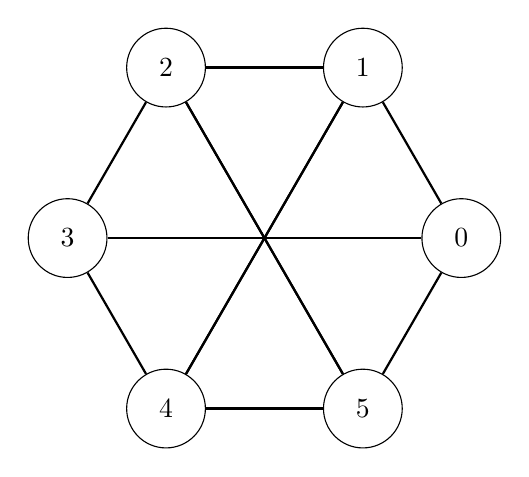
\begin{tikzpicture}
	\foreach \x in {0,1,2,3,4,5} {
	  \node[circle,draw,minimum size=10mm] (\x) at (\x*60:2.5) {\x};
    }

    \foreach \x in {0,1,2,3,4,5} {
	  \pgfmathtruncatemacro{\y}{mod(\x+1,6)}
	  \draw[thick] (\x) -- (\y);
    }

    \foreach \x in {0,1,2,3,4,5} {
	  \pgfmathtruncatemacro{\y}{mod(\x+3,6)}
	  \draw[thick] (\x) -- (\y);
    }
  \end{tikzpicture}
  \caption{Cayley graph of $\Z_6$}%
  \label{fig:sg-03-cayley-z6}
\end{figure}

Note that two elements $x, y \in G$ are adjacent in $\Cay(G,S)$ if and only if
$yx^{-1} \in S$.
The neighbourhood of a vertex is then
\[
  \Cay(G,S)(x) = \{ sx \such s \in S \},
\]
where we used the notation $\Gamma(x) = N_\Gamma(x)$.
In particular, $\Cay(G,S)$ is an $\abs{S}$-regular graph.

% LocalWords:  Cayley
